\documentclass{standalone}
\usepackage{tikz}
\usetikzlibrary{patterns, positioning}

\begin{document}
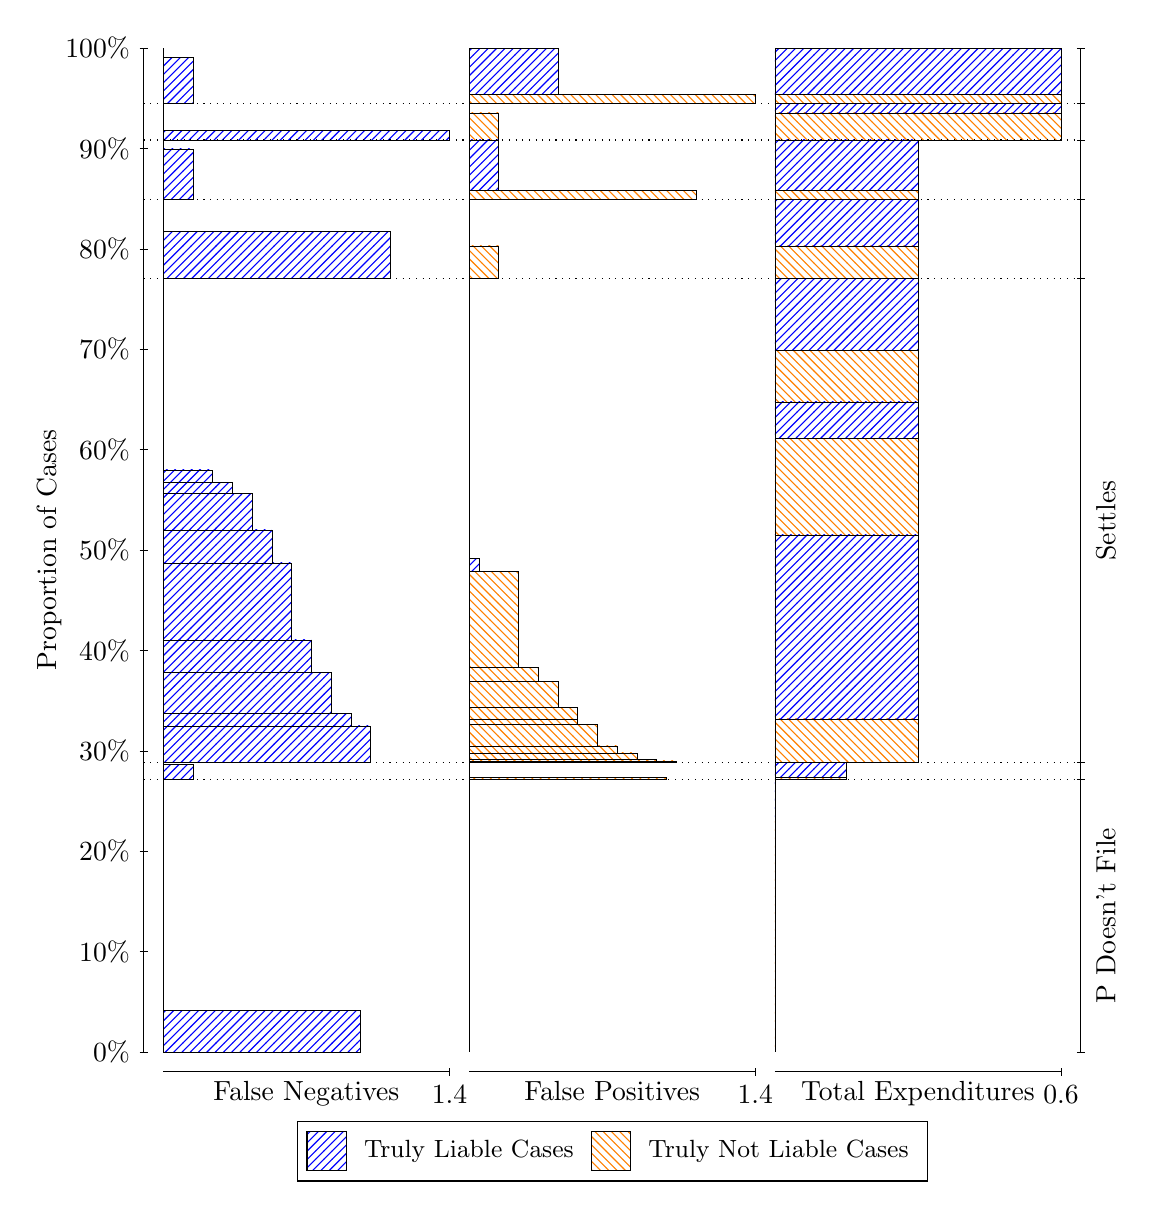
\begin{tikzpicture}
\draw[black, very thin] (1.5,1.75) -- (1.5,14.5);
\node[rotate=90, anchor=center] at (0.3, 8.125) {Proportion of Cases};
\draw[black, very thin] (1.45,1.75) -- (1.55,1.75);
\node[anchor=east] at (1.45, 1.75) {0\%};
\draw[black, very thin] (1.45,3.025) -- (1.55,3.025);
\node[anchor=east] at (1.45, 3.025) {10\%};
\draw[black, very thin] (1.45,4.3) -- (1.55,4.3);
\node[anchor=east] at (1.45, 4.3) {20\%};
\draw[black, very thin] (1.45,5.575) -- (1.55,5.575);
\node[anchor=east] at (1.45, 5.575) {30\%};
\draw[black, very thin] (1.45,6.85) -- (1.55,6.85);
\node[anchor=east] at (1.45, 6.85) {40\%};
\draw[black, very thin] (1.45,8.125) -- (1.55,8.125);
\node[anchor=east] at (1.45, 8.125) {50\%};
\draw[black, very thin] (1.45,9.4) -- (1.55,9.4);
\node[anchor=east] at (1.45, 9.4) {60\%};
\draw[black, very thin] (1.45,10.675) -- (1.55,10.675);
\node[anchor=east] at (1.45, 10.675) {70\%};
\draw[black, very thin] (1.45,11.95) -- (1.55,11.95);
\node[anchor=east] at (1.45, 11.95) {80\%};
\draw[black, very thin] (1.45,13.225) -- (1.55,13.225);
\node[anchor=east] at (1.45, 13.225) {90\%};
\draw[black, very thin] (1.45,14.5) -- (1.55,14.5);
\node[anchor=east] at (1.45, 14.5) {100\%};

\draw[black, very thin] (13.4,1.75) -- (13.4,14.5);
\draw[black, very thin] (13.35,1.75) -- (13.45,1.75);
\node[anchor=west] at (13.35, 1.75) {};
\draw[black, very thin] (13.35,5.213) -- (13.45,5.213);
\node[anchor=west] at (13.35, 5.213) {};
\draw[black, very thin] (13.35,5.4231) -- (13.45,5.4231);
\node[anchor=west] at (13.35, 5.4231) {};
\draw[black, very thin] (13.35,11.577) -- (13.45,11.577);
\node[anchor=west] at (13.35, 11.577) {};
\draw[black, very thin] (13.35,12.579) -- (13.45,12.579);
\node[anchor=west] at (13.35, 12.579) {};
\draw[black, very thin] (13.35,13.332) -- (13.45,13.332);
\node[anchor=west] at (13.35, 13.332) {};
\draw[black, very thin] (13.35,13.794) -- (13.45,13.794);
\node[anchor=west] at (13.35, 13.794) {};
\draw[black, very thin] (13.35,14.5) -- (13.45,14.5);
\node[anchor=west] at (13.35, 14.5) {};

\draw[black, very thin, pattern color=blue, pattern=north east lines] (1.75,1.75) rectangle (4.2557,2.2805);
\draw[black, very thin, pattern color=orange, pattern=north west lines] (1.75,2.2805) rectangle (1.75,5.213);
\draw[black, very thin, pattern color=blue, pattern=north east lines] (1.75,5.213) rectangle (2.1259,5.4024);
\draw[black, very thin, pattern color=orange, pattern=north west lines] (1.75,5.4024) rectangle (1.75,5.4231);
\draw[black, very thin, pattern color=blue, pattern=north east lines] (1.75,5.4231) rectangle (4.381,5.8913);
\draw[black, very thin, pattern color=blue, pattern=north east lines] (1.75,5.8913) rectangle (4.1305,6.0549);
\draw[black, very thin, pattern color=blue, pattern=north east lines] (1.75,6.0549) rectangle (3.8799,6.5749);
\draw[black, very thin, pattern color=blue, pattern=north east lines] (1.75,6.5749) rectangle (3.6293,6.9841);
\draw[black, very thin, pattern color=blue, pattern=north east lines] (1.75,6.9841) rectangle (3.3787,7.962);
\draw[black, very thin, pattern color=blue, pattern=north east lines] (1.75,7.962) rectangle (3.1282,8.3816);
\draw[black, very thin, pattern color=blue, pattern=north east lines] (1.75,8.3816) rectangle (2.8776,8.8442);
\draw[black, very thin, pattern color=blue, pattern=north east lines] (1.75,8.8442) rectangle (2.627,8.9803);
\draw[black, very thin, pattern color=blue, pattern=north east lines] (1.75,8.9803) rectangle (2.3764,9.1417);
\draw[black, very thin, pattern color=orange, pattern=north west lines] (1.75,9.1417) rectangle (1.75,11.577);
\draw[black, very thin, pattern color=blue, pattern=north east lines] (1.75,11.577) rectangle (4.6316,12.167);
\draw[black, very thin, pattern color=orange, pattern=north west lines] (1.75,12.167) rectangle (1.75,12.579);
\draw[black, very thin, pattern color=blue, pattern=north east lines] (1.75,12.579) rectangle (2.1259,13.22);
\draw[black, very thin, pattern color=orange, pattern=north west lines] (1.75,13.22) rectangle (1.75,13.332);
\draw[black, very thin, pattern color=blue, pattern=north east lines] (1.75,13.332) rectangle (5.3833,13.451);
\draw[black, very thin, pattern color=orange, pattern=north west lines] (1.75,13.451) rectangle (1.75,13.794);
\draw[black, very thin, pattern color=blue, pattern=north east lines] (1.75,13.794) rectangle (2.1259,14.379);
\draw[black, very thin, pattern color=orange, pattern=north west lines] (1.75,14.379) rectangle (1.75,14.5);
\draw[black, very thin, pattern color=orange, pattern=north west lines] (5.6333,1.75) rectangle (5.6333,4.6824);
\draw[black, very thin, pattern color=blue, pattern=north east lines] (5.6333,4.6824) rectangle (5.6333,5.213);
\draw[black, very thin, pattern color=orange, pattern=north west lines] (5.6333,5.213) rectangle (8.1391,5.2337);
\draw[black, very thin, pattern color=blue, pattern=north east lines] (5.6333,5.2337) rectangle (5.6333,5.4231);
\draw[black, very thin, pattern color=orange, pattern=north west lines] (5.6333,5.4231) rectangle (8.2644,5.4454);
\draw[black, very thin, pattern color=orange, pattern=north west lines] (5.6333,5.4454) rectangle (8.0138,5.4695);
\draw[black, very thin, pattern color=orange, pattern=north west lines] (5.6333,5.4695) rectangle (7.7632,5.5498);
\draw[black, very thin, pattern color=orange, pattern=north west lines] (5.6333,5.5498) rectangle (7.5126,5.6382);
\draw[black, very thin, pattern color=orange, pattern=north west lines] (5.6333,5.6382) rectangle (7.2621,5.9118);
\draw[black, very thin, pattern color=orange, pattern=north west lines] (5.6333,5.9118) rectangle (7.0115,5.9794);
\draw[black, very thin, pattern color=orange, pattern=north west lines] (5.6333,5.9794) rectangle (7.0115,6.1258);
\draw[black, very thin, pattern color=orange, pattern=north west lines] (5.6333,6.1258) rectangle (6.7609,6.4542);
\draw[black, very thin, pattern color=orange, pattern=north west lines] (5.6333,6.4542) rectangle (6.5103,6.6377);
\draw[black, very thin, pattern color=orange, pattern=north west lines] (5.6333,6.6377) rectangle (6.2598,7.8583);
\draw[black, very thin, pattern color=blue, pattern=north east lines] (5.6333,7.8583) rectangle (5.7586,8.0197);
\draw[black, very thin, pattern color=blue, pattern=north east lines] (5.6333,8.0197) rectangle (5.6333,11.577);
\draw[black, very thin, pattern color=orange, pattern=north west lines] (5.6333,11.577) rectangle (6.0092,11.988);
\draw[black, very thin, pattern color=blue, pattern=north east lines] (5.6333,11.988) rectangle (5.6333,12.579);
\draw[black, very thin, pattern color=orange, pattern=north west lines] (5.6333,12.579) rectangle (8.5149,12.69);
\draw[black, very thin, pattern color=blue, pattern=north east lines] (5.6333,12.69) rectangle (6.0092,13.332);
\draw[black, very thin, pattern color=orange, pattern=north west lines] (5.6333,13.332) rectangle (6.0092,13.675);
\draw[black, very thin, pattern color=blue, pattern=north east lines] (5.6333,13.675) rectangle (5.6333,13.794);
\draw[black, very thin, pattern color=orange, pattern=north west lines] (5.6333,13.794) rectangle (9.2667,13.915);
\draw[black, very thin, pattern color=blue, pattern=north east lines] (5.6333,13.915) rectangle (6.7609,14.5);
\draw[black, very thin, pattern color=orange, pattern=north west lines] (9.5167,1.75) rectangle (9.5167,4.6824);
\draw[black, very thin, pattern color=blue, pattern=north east lines] (9.5167,4.6824) rectangle (9.5167,5.213);
\draw[black, very thin, pattern color=orange, pattern=north west lines] (9.5167,5.213) rectangle (10.425,5.2337);
\draw[black, very thin, pattern color=blue, pattern=north east lines] (9.5167,5.2337) rectangle (10.425,5.4231);
\draw[black, very thin, pattern color=orange, pattern=north west lines] (9.5167,5.4231) rectangle (11.333,5.9794);
\draw[black, very thin, pattern color=blue, pattern=north east lines] (9.5167,5.9794) rectangle (11.333,8.3179);
\draw[black, very thin, pattern color=orange, pattern=north west lines] (9.5167,8.3179) rectangle (11.333,9.5384);
\draw[black, very thin, pattern color=blue, pattern=north east lines] (9.5167,9.5384) rectangle (11.333,10.007);
\draw[black, very thin, pattern color=orange, pattern=north west lines] (9.5167,10.007) rectangle (11.333,10.665);
\draw[black, very thin, pattern color=blue, pattern=north east lines] (9.5167,10.665) rectangle (11.333,11.577);
\draw[black, very thin, pattern color=orange, pattern=north west lines] (9.5167,11.577) rectangle (11.333,11.988);
\draw[black, very thin, pattern color=blue, pattern=north east lines] (9.5167,11.988) rectangle (11.333,12.579);
\draw[black, very thin, pattern color=orange, pattern=north west lines] (9.5167,12.579) rectangle (11.333,12.69);
\draw[black, very thin, pattern color=blue, pattern=north east lines] (9.5167,12.69) rectangle (11.333,13.332);
\draw[black, very thin, pattern color=orange, pattern=north west lines] (9.5167,13.332) rectangle (13.15,13.675);
\draw[black, very thin, pattern color=blue, pattern=north east lines] (9.5167,13.675) rectangle (13.15,13.794);
\draw[black, very thin, pattern color=orange, pattern=north west lines] (9.5167,13.794) rectangle (13.15,13.915);
\draw[black, very thin, pattern color=blue, pattern=north east lines] (9.5167,13.915) rectangle (13.15,14.5);
\draw[black, dotted] (1.5,5.213) -- (13.4,5.213);
\draw[black, dotted] (1.5,5.4231) -- (13.4,5.4231);
\draw[black, dotted] (1.5,11.577) -- (13.4,11.577);
\draw[black, dotted] (1.5,12.579) -- (13.4,12.579);
\draw[black, dotted] (1.5,13.332) -- (13.4,13.332);
\draw[black, dotted] (1.5,13.794) -- (13.4,13.794);
\draw[black, very thin] (1.75,1.5) -- (5.3833,1.5);
\node[anchor=north] at (3.5667, 1.5) {False Negatives};
\draw[black, very thin] (5.3833,1.45) -- (5.3833,1.55);
\node[anchor=north] at (5.3833, 1.45) {1.4};

\draw[black, very thin] (5.6333,1.5) -- (9.2667,1.5);
\node[anchor=north] at (7.45, 1.5) {False Positives};
\draw[black, very thin] (9.2667,1.45) -- (9.2667,1.55);
\node[anchor=north] at (9.2667, 1.45) {1.4};

\draw[black, very thin] (9.5167,1.5) -- (13.15,1.5);
\node[anchor=north] at (11.333, 1.5) {Total Expenditures};
\draw[black, very thin] (13.15,1.45) -- (13.15,1.55);
\node[anchor=north] at (13.15, 1.45) {0.6};

\node[black, centered, rotate=90] at (13.72, 3.4815) {P Doesn't File};

\node[black, centered, rotate=90] at (13.72, 8.5) {Settles};





\draw (7.449999999999999,1.5) node[draw=none] (baseCoordinate) {};
\begin{scope}[align=center]
        \matrix[scale=0.5, draw=black, below=0.5cm of baseCoordinate, nodes={draw}, column sep=0.1cm]{
            \node[rectangle, draw, minimum width=0.5cm, minimum height=0.5cm, pattern=north east lines, pattern color=blue] {}; &
            \node[draw=none, font=\small] (B) {Truly Liable Cases}; &
            \node[rectangle, draw, minimum width=0.5cm, minimum height=0.5cm, pattern=north west lines, pattern color=orange] {}; &
            \node[draw=none, font=\small] (B) {Truly Not Liable Cases}; \\
            };
\end{scope}

\end{tikzpicture}
\end{document}